\global\long\def\ys{\varphi}%

\global\long\def\im{\text{Im}}%


\section{线性空间的基本概念}

我们研究问题是从具体到抽象的, 从特殊到一般的, 于是自然就要考虑一下我们以前探讨过的多项式, 矩阵, 和普通的数在操作有什么共通的地方. 

我们先来考虑加法的共性. 得到了$V1\sim V4$. 

然后考虑减法的共性, 这时候就要依赖一个数域F, 得到了$V6\sim V8$.

其中$V5$在这里好像不是必须的, 因为我们可以从其他的几条性质里面推导出来. 

但是这八条性质有更加深刻的意义. $V2+V3+V4=\lyxmathsym{群的定义}$, $V1+\lyxmathsym{群的定义}=\lyxmathsym{交换群的定义}$,
$V5+V6+V7+V8=\lyxmathsym{模的定义}$. 注意我们在写定义的时候不要用上交换律的性质: 在左边都在左边,
在右边都在右边. 
\begin{defn}
(线性空间的八条性质) 设$V$是一个非空集合, $\F$是一个数域, 在$V$中定义了一个一种运算, 成为\textbf{加法},
即, 对于任意的$\alpha,$$\beta\in V$, 存在唯一的元素$\gamma\in V$与之对应, 记作$\gamma=\alpha+\beta$.
在$\F$与$V$之间定义了一个运算, 存在唯一的元素$\gamma\in V$与之对应, TODO
\end{defn}

\section{线性空间的基与维数}

在之前的内容中, 我们了解了线性空间的定义. 在之前我们做的事情就是做线性组合, 形式化的我们给出定义: 
\begin{defn}
(线性组合) TODO
\end{defn}
我们来举一些例子:
\begin{example}
(有限维多项式)
\end{example}
%
\begin{example}
(矩阵多项式) 如果$A\in\F^{n\times n}$, $f(x)\in\F[x],f(x)=a_{o}x_{0}+a_{1}x^{1}+\cdots+a_{n}x^{n}$,
如果对$f(x)$赋值为一个矩阵$f(A)=a_{0}I_{n}+a_{1}A+a_{2}A^{2}+\cdots+a_{n}A^{n}$,
问是否存在$f(A)=0,$也就是$I_{n},A,\cdots,A^{n}$的线性组合为0?
\end{example}
回顾上面两个例子, 我们为了刻画这种关系, 来描述\textbf{线性相关性}如下:
\begin{defn}
(线性相关性)
\end{defn}
\begin{example}
(平面向量, 空间向量的线性相关和线性无关)
\end{example}
我们希望找到一些最少的向量把空间``撑起来'', 于是我们给出如下的定义:
\begin{defn}
(极大线性无关组)
\end{defn}
如何求解极大线性无关组呢? 我们可以使用\textbf{筛选法}. 
\begin{defn}
(筛选法)
\end{defn}
运用筛选法得到的极大线性无关组是不唯一的, 但是筛选得到的元素的个数是唯一的. 我们把它定义为这个向量组的\textbf{秩}.
\begin{defn}
(基与维数) 设$V_{/\F}$, 若$\alpha_{1}..\alpha_{n}\in V$且线性无关, 且$\forall\alpha\in V$都可以用$\alpha_{1}..\alpha_{n}$\textbf{的线性组合表出},
则称$\alpha_{1}..\alpha_{n}$为$V$的一组基. 称$n$为$V/\F$的维数. 
\end{defn}
\begin{example}
平面是2维的, 空间是3维的. 
\end{example}
\begin{thm}
\label{base-represent-ok}若$\beta_{1}..\beta_{n}$是$V$的一组基, 则$\beta_{1}..\beta_{n}$与$\alpha_{1}..\alpha_{n}$线性等价且可以互相表出$\Rightarrow$$n=m$. 
\end{thm}
\begin{proof}
由于$\beta_{1}..\beta_{m}$可以与$\alpha_{1}..\alpha_{n}$线性等价, 我们可以得到这样的方程组,
其中$a_{11}..a_{mn}$是常数: 

\[
\begin{cases}
\beta_{1}= & a_{11}\alpha_{1}+..+a_{1n}\alpha_{n}\\
\beta_{2}= & a_{21}\alpha_{1}+..+a_{2n}\alpha_{n}\\
\vdots & \vdots\\
\beta_{m}= & a_{m1}\alpha_{1}+..+a_{mn}\alpha_{n}
\end{cases}
\]

由于这个记号看起来非常的难看, 我们不妨考虑简化记号: 比如
\[
\sum_{i=1}^{n}a_{i}b_{i}=\begin{pmatrix}a_{1}\\
a_{2}\\
\vdots\\
a_{n-1}\\
a_{n}
\end{pmatrix}\begin{pmatrix}b_{1} & b_{2} & \cdots & b_{n-1} & b_{n}\end{pmatrix}
\]

用上这个表示技巧, 我们就可以把$\beta_{1}$表示为如下所示的内容. 注意, $(\alpha_{1}..\alpha_{n})$只是形式上的行向量,
每一个$\alpha_{1}\cdots\alpha_{n}$其实上是一个列向量. 后面的内容才是真正在$\F^{n\times1}$中的元素.

\begin{align*}
\beta_{1}= & \begin{pmatrix}\alpha_{1} & \cdots & \alpha_{n}\end{pmatrix}\begin{pmatrix}a_{11}\\
\vdots\\
a_{1n}
\end{pmatrix}\\
\beta_{2}= & \begin{pmatrix}\alpha_{1} & \cdots & \alpha_{n}\end{pmatrix}\begin{pmatrix}a_{21}\\
\vdots\\
a_{2n}
\end{pmatrix}\\
\cdots & \cdots\\
\beta_{m}= & \begin{pmatrix}\alpha_{1} & \cdots & \alpha_{n}\end{pmatrix}\begin{pmatrix}a_{m1}\\
\vdots\\
a_{mn}
\end{pmatrix}
\end{align*}

于是考虑把上述的内容组合到一起:

\[
(\beta_{1},\beta_{2},\cdots,\beta_{m})=(\alpha_{1},\alpha_{2},\cdots,\alpha_{n})\begin{pmatrix}a_{11} & a_{12} & \cdots & a_{1n}\\
\cdots &  &  & \vdots\\
a_{m1} & a_{m2} & \cdots & a_{mn}
\end{pmatrix}
\]

分类讨论:
\begin{casenv}
\item 若$n\neq m$, 
\begin{casenv}
\item 若$n<m$, $A\in\F^{n\times m},AX=0,$说明一定存在非零解$\eta\in\F^{m\times1}$成立.
证明如下: 

\[
\left(\beta_{1}..\beta_{n}\right)=\left(\alpha_{1}..\alpha_{n}\right)A
\]

两端同时右乘$\eta$, 有$\left(\beta_{1}..\beta_{n}\right)\eta=\left(\left(\alpha_{1}..\alpha_{n}\right)A\right)\eta$.
可以证明形式矩阵的乘法具有结合律, 于是有$\left(\beta_{1}..\beta_{n}\right)\eta=\left(\alpha_{1}..\alpha_{n}\right)\left(A\eta\right)$,
而$A\eta=0$, 说明$\beta_{1}..\beta_{n}$线性相关, 矛盾!
\item $n<m$, 同理. 
\end{casenv}
\item $n=m,$由于自然数的三歧性, 维数存在, 说明$n=m$成立. 
\end{casenv}
\end{proof}
%
\noindent\shadowbox{\begin{minipage}[t]{1\columnwidth - 2\fboxsep - 2\fboxrule - \shadowsize}%
上例中形式矩阵具有结合律的一个证明:

\begin{align*}
\left(\begin{pmatrix}\alpha_{1} & .. & \alpha_{n}\end{pmatrix}A\right)\eta & = & \left(\begin{pmatrix}\alpha_{1} & .. & \alpha_{n}\end{pmatrix}\begin{pmatrix}a_{11} & .. & a_{1m}\\
\vdots &  & \vdots\\
a_{n1} & .. & a_{nm}
\end{pmatrix}\right)\begin{pmatrix}\eta_{1}\\
\vdots\\
\eta_{n}
\end{pmatrix}\\
 & = & \left(\begin{pmatrix}\alpha_{1} & .. & \alpha_{n}\end{pmatrix}\begin{pmatrix}a_{11}\\
\vdots\\
a_{n1}
\end{pmatrix},..,\begin{pmatrix}\alpha_{1} & .. & \alpha_{n}\end{pmatrix}\begin{pmatrix}a_{1m}\\
\vdots\\
a_{nm}
\end{pmatrix}\right)\begin{pmatrix}\eta_{1}\\
\vdots\\
\eta_{n}
\end{pmatrix}\\
 & = & \left(\begin{pmatrix}\alpha_{1} & .. & \alpha_{n}\end{pmatrix}\begin{pmatrix}a_{11}\\
\vdots\\
a_{n1}
\end{pmatrix}\right)\eta_{1}+..+\left(\begin{pmatrix}\alpha_{1} & .. & \alpha_{n}\end{pmatrix}\begin{pmatrix}a_{1m}\\
\vdots\\
a_{nm}
\end{pmatrix}\right)\eta_{n}\\
 & = & \left(\begin{pmatrix}\alpha_{1} & .. & \alpha_{n}\end{pmatrix}\begin{pmatrix}\eta_{1}a_{11}\\
\vdots\\
\eta_{1}a_{n1}
\end{pmatrix}\right)+..+\left(\begin{pmatrix}\alpha_{1} & .. & \alpha_{n}\end{pmatrix}\begin{pmatrix}\eta_{n}a_{1m}\\
\vdots\\
\eta_{n}a_{nm}
\end{pmatrix}\right)\\
 & = & \begin{pmatrix}\alpha_{1} & .. & \alpha_{n}\end{pmatrix}\left(A\eta\right)
\end{align*}
%
\end{minipage}}

类似于平面几何和立体几何, 我们也希望有一个坐标来更好的研究线性空间, 于是我们给出坐标的定义:
\begin{defn}
(坐标)
\end{defn}
可以验证, 在基给定的情形下, 坐标是唯一确定的. 从\ref{base-represent-ok}可以看出, 每组基的元素个数是相等的.
也就是
\begin{thm}
若$\alpha_{1}..\alpha_{n}$是线性空间V上的一组基, $\beta_{1}..\beta_{m}$也是$V$上的一组基,
则m=n. 
\end{thm}
那么我们自然的会想到有时候基不是很方便, 我们希望得到一个更加方便的基底, 这样我们就可以更好的考察这个线性空间的若干性质. 所以我们定义\textbf{过渡矩阵}.
通过右乘一个这样的矩阵, 我们可以顺利的把基进行变换. 那么, 要变成什么样的矩阵比较好呢? 实际上, 这样的矩阵会在下一章讲解线性变换的时候有大用处,
并且还会定义一个方阵的特征值和特征向量. 
\begin{defn}
(过渡矩阵) 我们可以使用右乘过渡矩阵方法完成基的变换. 设$\alpha_{1}..\alpha_{n}$和$\beta_{1},..,\beta_{n}$是$V$上的两组基,
有 

\[
\left(\beta_{1}..\beta_{n}\right)=\left(\alpha_{1}..\alpha_{n}\right)\begin{pmatrix}a_{11} & .. & a_{1n}\\
\vdots &  & \vdots\\
a_{n1} & .. & a_{nn}
\end{pmatrix}:=\left(\alpha_{1}..\alpha_{n}\right)\left(T_{1}..T_{n}\right)
\]

称$\begin{pmatrix}a_{11} & .. & a_{1n}\\
\vdots &  & \vdots\\
a_{n1} & .. & a_{nn}
\end{pmatrix}$是从$\left(\alpha_{1}..\alpha_{n}\right)$到$\left(\beta_{1}..\beta_{n}\right)$的\textbf{过渡矩阵}.
并且$T_{j}$是$\beta_{j}$在$\alpha_{1}..\alpha_{n}$下的坐标. 
\end{defn}
\begin{thm}
上述过渡矩阵一定可逆. 
\end{thm}
\begin{proof}
如果过渡矩阵不可逆, 意味着$AX=0$存在非零解答, 左右两边同时右乘非零解, 矛盾. 
\end{proof}
\begin{lem}
下列命题等价:
\begin{itemize}
\item $V$为$n(n<\infty)$维线性空间
\item $\alpha_{1}..\alpha_{n}$是一组基底
\item $\forall\alpha\in V$都可以被$\alpha_{1}..\alpha_{n}$线性表出
\end{itemize}
\end{lem}
\begin{problem}
如果$A\in\F^{n\times n}$, 是否存在$f(x)\in\F[x],$使得$f(A)=0$, 但是$a_{i}$不全为0?
\end{problem}
线性变换中, 在哪个数域上面看也是不可少的. 有时候在一个数域上面看是线性空间, 在另一个数域上面看就不是了. 下面来举几个例子.
\begin{example}
$\mathbb{Q}(\sqrt{2})=\{a+b\sqrt{2}|a,b\in\mathbb{Q}\}$, $\mathbb{Q}(\sqrt{2})$既可以看作有理数域上的线性空间,
又可以看作自身的线性空间, 即$\mathbb{Q}(\sqrt{2})_{/\mathbb{Q}(\sqrt{2})}$.
\end{example}
\begin{thm}
$\text{\ensuremath{\mathbb{F}\subseteq\mathbb{K}\subseteq\mathbb{E}}}$是数域,
$\text{dim}\mathbb{E}/\mathbb{F}=\text{dim}\mathbb{E}/\mathbb{\mathbb{K}}\cdot\text{dim}\mathbb{\mathbb{K}}/\mathbb{F}$.
\end{thm}

\section{线性同构和线性映射}

回忆我们曾经提到过的线性空间, 有加法和数乘. 线性空间中的一个元素$\alpha$都可以用这个线性空间的一组基以及他们前面搭配上对应的系数(在给定的数域中)来表示.
比如$\alpha=a_{1}\alpha_{1}+\cdots+a_{n}\alpha_{n}$. 并且在上一节中我们也定义了坐标的概念.
那么, 是不是空间里面的所有的元素都能用坐标表示呢? 你可能会觉得这是显然可以的. 下面来简单看一下这方面的更深层次的内涵. 

我们知道, 如果在$\F$上的$n$维线性空间里面, 如果$\alpha_{1}..\alpha_{n}$是一组基, $\forall\alpha\in V,\exists!x_{1}..x_{n}\in\F,$有下图关系的映射: 

\[
\begin{array}{cccc}
\boldsymbol{\alpha} & = & \boldsymbol{x_{1}a_{1}+..} & \boldsymbol{+x_{n}a_{n}}\\
 & = & (\alpha_{1}..\alpha_{n}) & \boldsymbol{\begin{pmatrix}x_{1}\\
\vdots\\
x_{n}
\end{pmatrix}}\\
\varphi:\boldsymbol{V} &  & \longrightarrow & \boldsymbol{\F}^{\boldsymbol{n\times1}}\\
\uparrow\in &  & \text{唯\text{一确定}}\\
\alpha &  & \longrightarrow & X=\varphi(\alpha)\\
\beta &  & \longrightarrow & Y=\varphi(\beta)\\
\alpha+\beta &  & \longrightarrow & X+Y=\varphi(\alpha)+\varphi(\beta)\\
k\alpha &  & \longrightarrow & kX=\varphi(k\alpha)
\end{array}
\]

为了看看我们定义的``坐标''是不是真正可以完成这些内容的转换, 我们自然要问这些问题:
\begin{enumerate}
\item $\varphi$是单射吗? 是的. 因为上节课中定理\ref{base-represent-ok}可以看出. 
\item $\varphi$是满射吗? 是的, 这是基的定义告诉我们的. 这样就推出了$\varphi$是双射. 
\item $\varphi$保持加法吗? 可以验证$\varphi(\alpha+\beta)=\varphi(\alpha)+\varphi(\beta)$.
\item $\varphi$保持数乘吗? 可以验证$\varphi(k\alpha)=k\varphi(\alpha)$.
\end{enumerate}
于是我们说, 在线性空间上, $\F^{1\times n}$与$V$没有差别. 

顺便提一句, 如果3, 4, 我们称这个映射为一个\textbf{线性映射}, 如果同时满足1, 2, 3, 4, 我们称之为一个\textbf{线性同构}. 
\begin{defn}
(线性映射)
\end{defn}
%
\begin{defn}
(线性映射) 记作$U\simeq V$
\end{defn}
\begin{problem}
如果$\dim V/\F=n,V\simeq\F^{n\times1}$, 并且$\dim U/\F=n,U\simeq\F^{n\times1},$问$V\simeq U$吗?
\end{problem}
或许答案是肯定的, 这时候我们只需要从$\F^{n\times1}$中转一下就可以了 . 具体的, 有:

\[
\xymatrix{V\ar[r]^{\varphi}\ar[dr]_{\psi^{-1}\circ\varphi} & \F^{n\times1}\ar[d]^{\psi^{-1}}\\
 & \ar[u]^{\psi}U
}
\]

上面的图示是我们的设想, 我们还有一些问题需要解答: 
\begin{enumerate}
\item $\psi^{-1}$存在吗? 由于上面是双射, 所以是存在的, 并且也为双射.
\item $\psi^{-1}\circ\varphi$也是双射吗? 是的, 因为两个映射都是双射.
\item 这个合成是线性的吗? 只需要证明$\psi^{-1}$是线性的, $\varphi$也是线性的, 两个线性映射的合成也设线性的就可以了. 
\end{enumerate}
\noindent\ovalbox{\begin{minipage}[t]{1\columnwidth - 2\fboxsep - 0.8pt}%
证明: $\psi^{-1}$是线性的

TODO

证明: 两个线性映射的合成是线性的.

TODO%
\end{minipage}}

我们发现线性同构也是一个等价关系, 也就是满足自反性, 对称性, 传递性. 
\begin{prop}
(线性同构是等价关系)
\end{prop}
至此我们可能要问一问为什么要引入线性空间. 毕竟在一个$\F^{n\times1}$的上面做事情也挺好的. 原因之一是很多时候很多空间难以处理.
例如这个空间:
\begin{example}
考虑$\R^{+}$, 定义$a\oplus b=ab,k\circ a=a^{k},k\in\R,a,b\in\R^{+}$.
现在求这个空间的维数. 
\end{example}
我们立刻发现这个空间的维数不是很好直接观察出来. 因为基就十分的难找. 这时候我们不妨使用$\ln,\exp$两个在这个空间下是线性的映射来看一看,
这样我们就看到了这个空间化为了$\R^{+}$, 因此这个空间的维数就是1. 

在无穷维的情况下, 考虑$\F^{1\times\infty}$是无法办到的. 这时候就需要我们直面这个抽象的线性空间了. 

下面我们来解决一个同样维数之间(不是无穷维)的映射, 单射与满射的问题. 因为之后的问题解决单射和满射可能不是很直接, 但是如果我们能得到两个空间维数相同,
那么单射和满射就等价了. 于是我们给出这个引理:
\begin{lem}
\label{finite-equal-dim-bij}考虑$\varphi:V\to U$, $V,U$均为$n$维的,
那么$\varphi$是单射$\Leftrightarrow$$\varphi$是满射. 
\end{lem}
\begin{proof}
记$\text{Im \ensuremath{\varphi}=\{\ensuremath{\varphi(\alpha)|\alpha\in V\}=\varphi(V)} ,}$TODO
\end{proof}
\begin{defn}
若$\varphi:V\to U$满足:
\begin{enumerate}
\item $\varphi(\alpha+\beta)=\varphi(\alpha)+\varphi(\beta)$
\item $\varphi(k\alpha)=k\varphi(\alpha)$
\end{enumerate}
就称其为\textbf{线性映射}. 记所有线性映射的全体为$\text{Hom}(V,U)$. 

\end{defn}
\begin{example}
(线性方程组)

我们知道可以把线性方程组写成如下的形式:

\[
AX=\beta,A\in\F^{m\times n},\beta\in F^{m\times1}
\]

如果\textbf{把左乘$A$看做一个映射}的话, 这个映射是把$\F^{n\times1}$映到了$\F^{m\times1}$了.
如果这样的映射我们记作$\varphi_{A}$的话, 那么$\varphi_{A}$是线性映射吗? 更具体的, 我们有如下的图示意:

\[
\xymatrix{V^{n}\ar[d]_{\simeq}\ar[r]^{\varphi} & U^{m}\ar[d]_{\simeq}\\
\F^{n\times1}\ar[r]_{\hat{\varphi}}^{\simeq} & \F^{m\times1}
}
\]

其中$\hat{\varphi}$一定形如某个$\varphi$. 下面我们来问几个问题:
\begin{enumerate}
\item $AX=\beta$有解吗? 答案与如下的内容等价: 
\begin{enumerate}
\item $r(A)=r(A|\beta)$
\item $\beta$可以被$A$的列向量线性表出. 
\end{enumerate}
就像在引理\ref{finite-equal-dim-bij}中的那样, 我们可以考虑把映射作用在空间里面所有可能矩阵之后的\textbf{像}放在集合里面,
称为\textbf{像集}, 也就是$\text{Im}\varphi_{A}=\{\varphi_{A}(x)|x\in\F^{n\times1}\}$,
类似于在函数中自变量跑遍所有可能的取值, 观察因变量的取值, 称为\textbf{值域}一样. 
\item 求$AX=0$的解. 

事实上, 这个解集是十分重要的. 也就是求$\{X\in\F^{n\times1}|\varphi_{A}(X)=0\}$, 我们很多时候把它叫做这个映射的\textbf{核}.
用记号$\ker\varphi_{A}$来表示上面的集合. \\
为什么核集合如此重要呢? 因为右侧从等于0到等于$\beta$是需要一点点变动, 也就是一个\textbf{特解}. 这样我们就可以得到所有的解集了. 
\item 求特解$\eta_{0}$, 也就是$A\eta_{0}=\beta$, 这样一来, $Ax=\beta$的所有解就都可以写作$\eta_{0}+\eta,\eta\in\ker\varphi_{A}$. 
\end{enumerate}
\end{example}
%
\begin{example}
(一个奇怪的例子, 和Lie群有关)
\end{example}
%
\begin{example}
(Lagrange插值公式)
\end{example}
%
\begin{example}
(求导)
\end{example}

\section{子空间}

\subsection{基本定义}

在上一节的例子中, 我们其实从求解线性方程组发现了一个比较一般的内容: 
\begin{example}
\label{eg:linear-eqs-system}$A\in\F^{m\times n},\beta\in\F^{m\times1},$求线性方程组$AX=\beta$的步骤是:
\begin{enumerate}
\item 探讨解的存在性;
\item 寻找$AX=0$的解空间$W$
\item $AX=0$的解空间为$n-r(A)$
\item $AX=\beta$的解集是$\{\eta_{0}+\alpha|\alpha\in W\}$, 并且有性质$\{\eta_{0}+\alpha|\alpha\in W\}\stackrel[-\eta_{0}]{+\eta_{0}}{\leftrightharpoons}W$.
\end{enumerate}
我们在使用线性映射的观点去看整个内容的时候发现这件事情是很有价值的. 于是我们给出映射的核与像的定义: 
\end{example}
\begin{defn}
(映射的核与像)
\end{defn}
一个自然的问题就是, 一个映射的核上面有什么的性质?更一般的, 线性映射的核与像是不是线性空间? 
\begin{lem}
如果$\varphi\in\text{Hom}(V,U)$, $\ker\varphi,\text{Im}\varphi$都是线性空间. 
\end{lem}
从上面的证明我们可以感受到, $\ker\varphi,\text{Im}\varphi$继承且保留了$V,U$之间的运算及其性质.
并且我们还可以感受到, $\text{Ker}\varphi\subset V,\text{Im}\varphi\subset U$.
于是我们给出如下的定义: 
\begin{defn}
若$V/\F$, \textbf{$W\subseteq V$是}非空子集, 若$W$中\textbf{对于$V$的}加法,
数乘也构成线性空间, 则称$W$为$V$的子空间. 
\end{defn}
在理解这个定义的时候要注意如下几点: 
\begin{enumerate}
\item 这个集合要是非空的
\item 这个集合要继承下来$W$中对于加法, 数乘的定义, 并且对加法, 数乘具有封闭性. 
\end{enumerate}
\begin{prop}
设$W$是$V/\F$的非空子集, 则下列条件等价:
\begin{itemize}
\item $W$为$V$的子空间
\item W对V中的加法和数乘封闭
\item $\forall\alpha,\beta\in W,k,l\in\F,k\alpha+l\beta\in W$
\end{itemize}
\end{prop}
那么, 有没有最小的子空间呢? 其实$\{0\}$永远是$V$平凡的子空间. 下面同样给出几个空间包含的例子. 
\begin{example}
(平面和三维空间)
\end{example}
%
\begin{example}
(多项式空间)
\end{example}
%
\begin{example}
(连续函数的空间)
\end{example}
%
那么, 核空间和像空间之间有什么联系呢? 还是看我们的线性方程组的例子开始. 对于一个线性方程组, $\dim\ker\varphi_{A}=n-r(A)$,
$\dim\text{Im}\varphi_{A}=r(A)$, 而把它们的维数加起来就有和$\F^{n\times1}$是等价的.
也就是$\dim\ker\varphi_{A}+\dim\text{Im}\varphi_{A}=\dim V$. 下面我们来给出这个内容的一个证明.
\begin{proof}
TODO
\end{proof}
更加广阔的, 我们是不是可以证明
\begin{prop}
\label{dim-sum-eq-all}若$\varphi:V\to U$是线性映射, $\dim\ker\varphi_{A}+\dim\text{Im}\varphi_{A}=\dim V$,
当V是有限维线性空间的时候. 
\end{prop}
这个命题我们会在\ref{subsec:insert-and-sum}和\ref{subsec:quotient-ready}两节给出不同角度的证明. 

\subsection{交与和\label{subsec:insert-and-sum}}

有了子空间, 我们自然希望寻求一组子空间的基底. 首先我们可能会猜测: 子空间的基也可能由原空间``继承''下来. 
\begin{problem}
设$\dim V=n,$$W$为$V$的子空间, \textbf{$W$}的一组基是$\alpha_{1}..\alpha_{k}$.
设$q_{1}..q_{n}$是$V$的一组基, 则取$\{q_{1}..q_{n}\}\cap W$是$W$的一组基吗?
\end{problem}
答案当然不是. 在平面上可以找到反例. 
\begin{example}
(平面上子空间)
\end{example}
因此这告诉我们应当从小空间往大找, 而不是大空间往小的找. 具体的, 我们有这个定理:
\begin{thm}
设$\dim V=n<\infty$, $W$为$V$的子空间, $W$的一组基可以扩充为$V$的一组基. 
\end{thm}
证明的思路大致是取$V$的一组基,$\beta_{1}..\beta_{n}$, 将$\alpha_{1}..\alpha_{k}\beta_{1}..\beta_{n}$放在一起,
然后做筛选法就可以了. 
\begin{problem}
(思考题) 若V是无穷维的, 子空间可以基的扩充的方法做吗?
\end{problem}
有了这样的想法, 我们就可以来证明命题\ref{dim-sum-eq-all}($\dim\ker\varphi_{A}+\dim\text{Im}\varphi_{A}=\dim V$).
证明如下:
\begin{proof}
取$\ker\varphi$的一组基$\alpha_{1}..\alpha_{k}$, 扩充一下成为$V$的一组基$:\alpha_{1}..\alpha_{k}..\alpha_{n}$.
其中$\varphi(\alpha_{k+1})..\varphi(\alpha_{n})$是$\text{Im}\varphi$的生成元(由它们线性组合得到$\text{Im}\varphi$的元素,
记作$L(\varphi(\alpha_{k+1})..\varphi(\alpha_{n}))$. )

问题转换为需要证明$\dim\text{Im}\varphi=n-k\Leftrightarrow\varphi(\alpha_{k+1})..\varphi(\alpha_{n})$是线性无关的.
也就是$l_{k+1}\varphi(\alpha_{k+1})+..+l_{n}\varphi(\alpha_{n})=0$是不是可以说明$l_{k+1}..l_{n}$全为0?
于是给出如下的证明:

$l_{k+1}\varphi(\alpha_{k+1})+..+l_{n}\varphi(\alpha_{n})=0$意味着$l_{k+1}\alpha_{k+1}+..+l_{n}\alpha_{n}=0\in\ker\varphi$,
也就是$l_{k+1}\alpha_{k+1}+..+l_{n}\alpha_{n}=l_{1}\alpha_{1}+..+l_{k}\alpha_{k}$
, 移动项有: $l_{k+1}\alpha_{k+1}+..+l_{n}\alpha_{n}-\left(l_{1}\alpha_{1}+..+l_{k}\alpha_{k}\right)=0$,
由于$l_{1}..l_{k}$的线性无关性, 可以知道$\varphi(\alpha_{k+1})..\varphi(\alpha_{n})$是线性无关的.
因此是$\text{Im}\varphi$中的一组基. 
\end{proof}
接下来我们来看线性映射的全体之间单射、满射之间的关系. 在这之前, 我们再次引入一下下列记号; 
\begin{defn}
(Hom记号) 设$\varphi:V\to U,\text{Hom}(V/\F,U/\F)$是所有从V到U的线性映射的全体. 可记作$\varphi\in\text{Hom}(V/\F,U/\F)$. 
\end{defn}
如何让这个线性映射是满射? 其实很简单, 只要把$U$这个集合缩小到$\text{Im}\varphi$就行了. 

那如何让这个线性映射是一个单射呢? 我们希望只要缩小$V$这个集合就行了. 具体的, 只要让每一个被映过去的元素只有一个就行了.
于是我们可以找到一个$V$的子集$W$. 可以验证这个$W$也是$V$的一个子空间. 

\[
\xymatrix{\ker\varphi\ar[r]^{\text{单射}} & V/\F\ar[r]^{\varphi}\ar[dr]_{\varphi} & U/\F\\
 & W\ar[u]^{\text{单射}}\ar[r]_{\varphi|_{W}} & \im\varphi
}
\]

上面这张图里面的下面那一条线就得到了一个新的映射. 一般叫做作\textbf{限制映射}. 如果我们考察这个映射的核空间的话, 也就是$\ker\varphi|_{W}=W\cap\ker\varphi$,
会发现这个集合里面只有0, 并且$\varphi(W)=\im\ys=\ys(V)$下面我们来说明这件事情. 
\begin{prop}
限制映射$\ys|_{W}$的核空间与空间$W$的交只有$\{0\}$, 且$\ys(W)=\im\ys=\ys(V)$. 
\end{prop}
\begin{proof}
$\forall\alpha\in V$, $\exists\beta\in W,$使得$\ys(\alpha)=\ys(\bt)$,
$r:=\ys(\alp-\bt)=0\implies\alp-\bt\in\ker\ys.$
\end{proof}
从上面的证明和命题中我们可以看出任意的一个$\alp\in V$可以被分解为$\beta\in W$和$\gamma\in\ker\ys$.
这个在后续会用到. 

下面来给出子空间的交的定义: 
\begin{defn}
(子空间的交) 设$V_{1},V_{2}$为$V$的子空间, 称$V_{1}\cap V_{2}$为$V_{1}$与$V_{2}$的交. 
\end{defn}
%
\begin{defn}
(子空间的和) 设$W_{1},W_{2}\subset V,W_{1}+W_{2}=\left\{ \alpha_{1}+\alpha_{2}|\alp_{1}\in W_{1},\alp_{2}\in W_{2}\right\} .$
\end{defn}
我们在比较熟悉的地方来举几个例子:
\begin{example}
(平面上子空间的交) 
\end{example}
%
\begin{example}
(两个子空间的维数和其和维数之间的关系)
\end{example}
%

\subsection{直和}

有了子空间的和的问题之后, 我们自然要考虑子空间的和和子空间的并是一回事吗? 它们的区别是什么? 
\begin{defn}
\label{direct-sum-def}(直和) 设$V_{1},V_{2}$都是$V$的子空间, 则下列条件等价:
\begin{enumerate}
\item $V_{1}\cap V_{2}=\{0\}$
\item $\dim(V_{1}+V_{2})=\dim V_{1}+\dim V_{2}$
\item $V_{1}$的一组基与$V_{2}$的一组基可以合并成$V_{1}+V_{2}$的一组基
\item $\forall\alp\in V_{1}+V_{2}$, $\alp_{1}\in V_{1},\alp_{2}\in V_{2}$,
$\alp$的分解式唯一. 
\item 零向量的分解式唯一
\end{enumerate}
若$V_{1},V_{2}$满足上述五条的任何一条, 则称$V_{1}+V_{2}$是$V_{1}+V_{2}$的直和, 通常记作

\[
V_{1}\oplus V_{2}.
\]
\end{defn}
最后我们用矩阵的例子来看一看``直和''.
\begin{example}
(矩阵的分类与直和)
\end{example}

\section{商空间}

\subsection{准备工作\label{subsec:quotient-ready}}

在开始之前, 请回顾一下直和的定义(定义\ref{direct-sum-def})和维数公式(命题\ref{dim-sum-eq-all}). 

其实命题\ref{dim-sum-eq-all}的维数公式是一个特殊情形, 我们可以给出如下的维数公式:
\begin{thm}
(维数公式) $\dim(V_{1}\cap V_{2})+\dim(V_{1}+V_{2})=\dim V_{1}+\dim V_{2}$.
\end{thm}
\begin{proof}
TODO
\end{proof}
有时候我们可能需要空间的一个补集, 于是我们需要如下的定义: 
\begin{defn}
(补子空间) $V_{1}$是的$V$子空间, 如果存在$V_{2}$, 使得$V_{1}\oplus V_{2}=V$,
称$V_{2}$为$V$的\textbf{补子空间}.
\end{defn}
下面我们来通过一个实际的例子来看一看以前我们的线性方程组的思想(例子\ref{eg:linear-eqs-system})是不是可以被抽象出来. 

回顾左乘$A$矩阵的例子实际上是$\ys_{A}:\F^{n\times1}\to\F^{m\times1}\ni\bt$, 那么步骤大概是这样的
\begin{enumerate}
\item $AX=\bt$有解$\iff\bt\in\im\ys_{A}$
\item 若有解, 先求特解$\eta_{0},A\eta_{0}=\beta$, 要求任意解, 必须先求$AX=0$的解, 也就是$\ker\ys_{A}$.
\item $AX=\bt$的解集为$\eta_{0}+\ker\ys_{A}$
\item 能否选取特解$\eta$, 使得特解的全体构成$\F^{n\times1}$的子空间?
\end{enumerate}
不妨设$AX=\bt_{0}$对应的解空间为$\eta_{0}+W$, $AX=\bt_{1}$对应的解空间为$\eta_{1}+W$.
那么$AX=\bt_{0}+\bt_{1}$对应的解空间为$\eta_{0}+\eta_{1}+W$, $AX=k\bt_{0}$的解空间为$k\eta_{0}+W$.
这是一件很好玩的事情. 

再继续之前, 先来看看我们都玩了些什么. 

\[
\xymatrix{\text{一些例子\ar[r]\ar[d]} & \text{线性空间}\ar[r]^{\text{同构}}\ar[d] & \text{\ensuremath{\F^{n\times1}}}\\
\text{齐次线性方程组}AX=0\ar[r]\ar[d] & \text{基与维数}\ar[r] & \text{坐标}\ar[u]\\
\text{线性方程组}\text{\ensuremath{AX=\beta}}\ar[r]\ar[dd] & \text{线性映射}\ar[r]\ar[dr] & \text{核\ar[dr]}\\
 &  & \text{像}\ar[r] & \text{子空间}\\
\text{特解与通解}
}
\]


\subsection{商空间}

商空间是从解线性方程组里面出来的. 加入$A\eta_{0}=\bt$成立, 且$\eta_{0}$是特解, 那么所有解就会形如$\eta_{0}+W=\{\eta_{0}+\alp|\alpha\in W\}$,
$AX=0$的解空间记作$W$. 这样的情形就像我们在平面上考虑一些平行线一样. 
\begin{example}
(平面上的平行线) 能不能把这些线分个类呢?

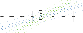
\includegraphics[scale=0.5]{figs/parallel-lines-on-plane}
\end{example}
还是从映射的角度考虑. 假设考虑$V(\F^{n\times1})\to U(\F^{m\times1}),(m<n)$的映射,
恰当的选取元素, 使得这是一个满射. 因为这样比较好考虑. 

\[
\begin{array}{ccccccccc}
\ys:V\to U\text{是满射} &  & (\ys_{A}: & \brokenvert & \F^{n\times1} & \to & \F^{m\times1} & (m<n) & )\\
 &  & \uparrow\in & \brokenvert & \varphi_{A}^{-1}(\bt) & \to & \bt\\
\text{有原象}\ys^{-1}(\beta_{1}) & \to & \text{给定}\beta_{1} & \brokenvert & \text{有原像}\varphi_{A}^{-1}(\beta) & \to & \text{给定}\beta\\
\text{有原象}\ys^{-1}(\beta_{2}) &  & \text{给定}\beta_{2} & \brokenvert & \text{(也就是} & Ax=B & \text{的解集)}\\
 &  &  & \brokenvert
\end{array}
\]

注意到每一个$\beta$总是对应\textbf{唯一的}一个原像. 并且原像构成的集合是$V$的一个子集. 因为不同的常数项在右边,
导致方程组的解集是不一样的. 也就是说
\begin{enumerate}
\item 若$\bt_{1}\neq\bt_{2}$, $\ys^{-1}(\bt_{1})\cap\ys^{-1}(\bt_{2})=\varnothing$.
\item $\forall\alpha\in V,\exists\bt,$使得$\alp\in\ys^{-1}(\bt)$. 只需要取得$\beta=\ys(\alp)$即可(取成0).
\item $V=\bigcup_{\beta\in U}\ys^{-1}(\bt)$, (由1是不交并).
\end{enumerate}
现在我们希望这个集合是单射, 因此, 不妨构造这样的一个集合$X$, 使得把映成同样元素的内容放在一起看. 这样构造的集合$X$与$U$之间的元素是一一对应的.
也就是

\[
X=\left\{ \varphi^{-1}(\bt)|\bt\in U\right\} \subseteq\mathsf{PSET}(U)
\]

$\mathsf{PSET}(U)$是$U$的幂集. 也就是$U$的所有子集构成的集合, 比如$\mathsf{PSET}(\{1,2,3\})=\{\{1\},\{2\},\{3\},\{1,2\},\{2,3\},\{1,3\},\{1,2,3\}\}.$
相关内容可以参看离散数学集合论相关的内容. 

那么这个集合性质很好, 我们能不能把$U$上的加法和数乘\textbf{平移到$X$上面去}?

\[
\xymatrix{\text{不知道怎么加}\rightarrow & \ys^{-1}(\bt_{1})\ar[d]^{\ys} & + & \ys^{-1}(\bt_{2})\ar[d]^{\ys} & \ys^{-1}(\bt_{1}+\bt_{2})\\
\text{映\text{射到这里}\ensuremath{\rightarrow}} & \bt_{1} & + & \bt_{2} & \bt_{1}+\bt_{2}\in U\ar[u]_{\text{映射回来}}^{\ys^{-1}}
}
\]

从上, 可以得到
\begin{itemize}
\item $X$是$\F$上面的线性空间.
\end{itemize}
这个$X$和$U,V$有什么关系呢? 

\noindent\fbox{\begin{minipage}[t]{1\columnwidth - 2\fboxsep - 2\fboxrule}%
\textbf{用$V$中的运算看$X$的运算:}

用原象的记号表达可能并不能让我们了解到底有什么联系. 我们具体的写一下: 

考虑这个线性空间中的一个特殊的元素零向量, 那么$\ys^{-1}(0)=\ker\ys$. 

令$W=\ker\ys\subset V$, 若$\ys(\alp)=\beta$, 考虑$\varphi^{-1}(\bt)={\alp+\gamma|\gamma\in W}$.
也就是可以通过特解和核空间里面的通解加起来得到. 简单记作$\alpha+W$.

如果$\ys(\alp_{1})=\bt_{1},\ys(\alp_{2})=\bt_{2},$由线性空间的性质, $\varphi^{-1}(\bt_{1})+\varphi^{-1}(\bt_{2})=\varphi^{-1}(\bt_{1}+\bt_{2})$,
有$\varphi^{-1}(\bt_{1})=\alp_{1}+W,\varphi^{-1}(\bt_{2})=\alp_{2}+W,\varphi^{-1}(\bt_{1})+\varphi^{-1}(\bt_{2})=\alp_{1}+\alp_{2}+W$.%
\end{minipage}}

由此我们可以发现:
\begin{thm}
若$\overline{\alp}\cap\overline{\bt}$非空, 则有下列条件:
\begin{enumerate}
\item $\bar{\alp}=\bar{\bt}$
\item $\alp-\bt\in W$
\item $\alp\in\bar{\bt}$
\item $\bt\in\bar{\alp}$
\end{enumerate}
\end{thm}
我们可以重新考虑一下这个子空间. 

\noindent\fbox{\begin{minipage}[t]{1\columnwidth - 2\fboxsep - 2\fboxrule}%
\textbf{$W\subset V$的子空间: }

$\forall\alp\in V,$考虑\textbf{子集}$\alp+W={\alp+\gamma|\gamma\in W}:=\bar{\alpha}$.
这样给定一个子空间之后, 通过改变$\gamma$的值, 就可以找到很多的子集. $V$也一定是这些子集的并集. 我们来考虑$\alp,\bt\in V$之间的元素的关系.
也就是

\[
\left.\begin{array}{ccccc}
V & \ni & \alpha & \rightarrow & \bar{\alpha}:=\alp+W\\
V & \ni & \beta & \rightarrow & \bar{\beta}:=\beta+W
\end{array}\right\} \text{\ensuremath{\bar{\alp}\cap\bar{\bt}=?}}
\]

假设存在$\delta=\alp+\gamma_{0}=\bt+\gamma_{1},$那么有$\alp-\bt=\gamma_{1}-\gamma_{0}\in W$,
$\alp=\bt+\gamma\in\bt+W$; $\beta=\alpha-\gamma\in\alpha+W$. 得到若$\bar{\alpha}\cap\bar{\bt}$非空,
那么$\alp=\bt$. 这样会被称作广义的平行. %
\end{minipage}}

在上述的这个子空间里面, 也有如下的一些性质可以满足: 

\noindent\fbox{\begin{minipage}[t]{1\columnwidth - 2\fboxsep - 2\fboxrule}%
\textbf{$W\subset V$的子空间:}

记$V/W=\{\alpha+W|\alp\in V\}$, 那么满足
\begin{enumerate}
\item 加法: $\alp+W+\bt+W=\alp+\bt+W$
\item 数乘: $(\alp+W)k=k\alp+W$.
\end{enumerate}
也就是简单记作$\bar{\alpha}+\bar{\bt}=\overline{\alpha+\beta},k\overline{\alpha}=\overline{k\alpha}$.

刚刚的内容让我们选取了一个代表元进行操作. 那么, 商空间的性质是不是和代表元的选取有关呢? 若更换$\alpha\leftarrow\alp_{1},\bt\leftarrow\bt_{1},$那么$\overline{\alp_{1}+\bt_{1}}=\overline{\alp+\bt}$成立吗?
如果要让定义合理的话, 这个要成立才可以. %
\end{minipage}}

在看到之前的问题的时候, 考虑如下的映射:

\[
\xymatrix{V\ar[r]^{\pi} & V/W\\
\alpha\ar[r] & \overline{\alpha}=\alpha+W
}
\]

并且记$\pi$作为\textbf{自然映射}. 那么这个映射有这些的性质:
\begin{enumerate}
\item $\pi$是满射
\item $\pi(\alp+\bt)=\overline{\alpha+\beta}=\bar{\alpha}+\bar{\bt}=\pi(\alp)+\pi(\bt)$
\item $\pi(k\alpha)=\overline{k\alpha}=k\overline{\alpha}=k\pi(\alpha)$
\item $\ker\varphi=W$
\item 取$V_{1}\subset V$是$W$的补子空间, 使得$\pi|_{V_{1}}:V_{1}\to V/W$是线性同构.
因为$V_{1}\cap\ker\pi=0,V_{1}+\ker\pi=V$, 意味着$W\oplus V_{1}=V$.
\item $V/W\simeq V_{1}\implies\dim V/W=\dim V-\dim W$. 注意: $V/W$不是$V$的子空间. 
\item 找到$V/W$的一组基$\iff$找到$W$的子空间的一组基, 记作$\alp_{1}..\alp_{k}$. 扩充为$V$的一组基:
$\alp_{1}..\alp_{k}\alp_{k+1}..\alp_{n}$, 则$L(\alp_{k+1}..\alp_{n})$为$W$的补子空间. 
\end{enumerate}
\begin{prop}
若$\pi(\alp_{1})=\overline{\alp_{1}},\pi(\alp_{2})=\overline{\alp_{2}},...,\pi(\alp_{k})=\overline{\alp_{k}},\pi(\alp_{k+1})=\overline{\alp_{k+1}}..,\pi(\alp_{n})=\overline{\alp_{n}}$,
$\overline{\alp_{1}}..\overline{\alp_{n}}$是商空间$V/W$的基.
\end{prop}
%
\begin{prop}
若$\overline{\alp_{1}}..\overline{\alp_{k}}\overline{\alp_{k+1}}..\overline{\alp_{n}}$,
$\overline{\alp_{1}}..\overline{\alp_{k}}$为$W$的一组基, 若$\alp_{1}..\alp_{k}$是$W$的一组基,
那么$\alp_{1}..\alp_{k}\alp_{k+1}..\alp_{n}$是$V$的一组基. 
\end{prop}
%
下面来说明基是不依赖于代表元的选取. 

(TODO)
\begin{example}
(在数列极限中的应用)
\end{example}
%
\begin{defn}
(等价关系)
\end{defn}

\section{线性代数中出现的内容}

\subsection{向量组以及其线性组合}

\global\long\def\vvec#1{(#1_{1},#1_{2},\cdots,#1_{n})}%

\global\long\def\lnvec#1#2{#1_{1},#1_{2},\cdots,#1_{#2}}%

\global\long\def\lsvec#1{#1_{1},#1_{2},\cdots,#1_{n}}%

\global\long\def\lgen#1#2#3{#1_{1}#2_{1}#3#1_{2}#2_{2}#3\cdots#3#1_{n}#2_{n}}%

\global\long\def\lngen#1#2#3{#1_{1}#2_{1}+#1_{2}#2_{2}+\cdots+#1_{#3}#2_{#3}}%

\begin{enumerate}
\item $n$维向量
\begin{enumerate}
\item 定义: $n$个数$\lsvec a$构成的有序数组$\vvec a^{T}$称为一个$n$维向量. 这$n$个数称为该向量的分量,
第$i$个数$a_{i}$称为这个向量的第$i$个分量. 
\item 运算:
\begin{enumerate}
\item 加法$\vvec a+\vvec b=(a_{1}+b_{1},a_{2}+b_{2},\cdots,a_{n}+b_{n})$
\item 数乘$k\vvec a=\vvec{ka},k\in\F$. 
\end{enumerate}
\end{enumerate}
\item 线性组合: 设$\lsvec{\boldsymbol{\alpha}}\in\F^{n},$$\lsvec k\in\F$, 那么$\lgen k{\boldsymbol{\alpha}}+$称为向量组$\vvec{\boldsymbol{\alpha}}$的一个线性组合.
\item 线性表示: 设$\boldsymbol{\beta}\in\R^{n}$, 若\textbf{存在}一组数$\lsvec k$,
使得$\beta=\lgen k{\boldsymbol{\alpha}}+,$那么称向量$\boldsymbol{\beta}$可以由$\boldsymbol{\alpha}$\textbf{线性表示}(\textbf{线性表出}).
\begin{enumerate}
\item Th. 向量$\beta$可以由$\lsvec{\boldsymbol{\alpha}}$线性表示的充分必要条件是矩阵$\boldsymbol{A}=\vvec{\boldsymbol{\alpha}}$和矩阵$\boldsymbol{A}=(\lsvec{\boldsymbol{\alpha}},\boldsymbol{\beta})$的秩相等. 
\end{enumerate}
\item 向量组的等价: 设$\boldsymbol{A}$和$\boldsymbol{B}$是两个向量组, 若向量组\textbf{$\boldsymbol{A}$}的\textbf{每个}向量都可以由向量组$\boldsymbol{B}$线性表示,
则称向量组$\boldsymbol{A}$可由向量组$\boldsymbol{B}$线性表示. 若向量组$\boldsymbol{A}$和向量组$\boldsymbol{B}$可以\textbf{互相线性表示},
则称向量组$\boldsymbol{A}$和向量组$\boldsymbol{B}$\textbf{等价}. 
\begin{enumerate}
\item Prop. 这是一个\textbf{等价关系}.
\begin{enumerate}
\item Coll. 向量组$\boldsymbol{A}$和$\boldsymbol{B}$等价的充要条件是$\rk{\boldsymbol{A}}=\rk{\boldsymbol{B}}=\rk{\boldsymbol{A},\boldsymbol{B}}$. 
\end{enumerate}
\end{enumerate}
\end{enumerate}

\subsection{向量组的线性相关性}
\begin{enumerate}
\item 线性相关与线性无关: 给定向量组$\boldsymbol{A}:\lsvec{\boldsymbol{\alpha}}(n\geq1)$,
如果\textbf{存在}一组\textbf{不全为0}的数$\lsvec k$, 使得$\lgen k{\boldsymbol{\alpha}}+=\boldsymbol{0}$,
则称向量组$\boldsymbol{A}$线性相关, 否则称向量组线性无关. 
\begin{enumerate}
\item 注: 这个命题的否定是$(\lgen k{\boldsymbol{\alpha}}+=\boldsymbol{0})\Longrightarrow(\forall\lsvec k=0)$.
可以参看离散数学中的命题逻辑一节学习. 
\end{enumerate}
\item 若干结论: 
\begin{enumerate}
\item 单独的一个非零向量线性无关
\item 如果一个向量组线性无关, 那么它的任何一个非空部分组也线性无关
\item 若$n$维向量$\lsvec{\boldsymbol{\alpha}}$组线性无关, 那么在相同的位置都添加一个分量之后得到的$n+1$维的向量组也线性无关. 
\item 若向量组$\lsvec{\boldsymbol{\alpha}}$线性无关, 但是$\lsvec{\boldsymbol{\alpha}},\boldsymbol{\beta}$线性相关,
则向量$\boldsymbol{\beta}$可由$\lsvec{\boldsymbol{\alpha}}$唯一线性表出. 
\item 如果一个向量组的一部分线性相关, 那么这个向量组线性相关
\item 如果向量组$(\circledast)\lsvec{\boldsymbol{\alpha}}$可由向量组$(\clubsuit)\lnvec{\boldsymbol{\beta}}r$线性表示,
且$\circledast$线性无关, 那么$\circledast$所含的向量个数不大于$\clubsuit$含的像两个数.
也就是$n\leq r$. 
\item 一个向量组线性相关$\Leftrightarrow$它所构成矩阵的秩\textbf{小于}向量个数; 一个向量组线性无关$\Leftrightarrow$它所构成矩阵的秩\textbf{等于}向量个数.
\end{enumerate}
\end{enumerate}

\subsection{向量组的秩}
\begin{enumerate}
\item 最大线性无关组
\begin{enumerate}
\item Def. %
\noindent\begin{minipage}[t]{1\columnwidth}%
给定向量组$\boldsymbol{A}$, 若存在$\boldsymbol{A}$的一个\textbf{部分组}$\boldsymbol{B}$:$\lnvec{\boldsymbol{\alpha}}s,$满足以下的两个条件:
\begin{itemize}
\item 向量组$\boldsymbol{B}$\textbf{线性无关}
\item 向量组$\boldsymbol{A}$中的\textbf{任意}$s+1$个向量\textbf{都能}由向量组$\boldsymbol{B}$线性表示
\end{itemize}
则称向量组$\boldsymbol{B}$是向量组$\boldsymbol{A}$的一个极大线性无关组. %
\end{minipage}
\item Prop.
\begin{enumerate}
\item 向量组与其最大线性无关组等价.
\item 一个向量组的最大线性无关组包含的个数是唯一的
\end{enumerate}
\end{enumerate}
\item 向量组的秩
\begin{enumerate}
\item Def. 向量组$\boldsymbol{A}$的最大线性无关组包含的向量个数称为向量组$\boldsymbol{A}$的秩.
规定只有零向量的向量组的秩为$0$.
\end{enumerate}
\item 矩阵的行秩和列秩
\begin{enumerate}
\item 分块: %
\noindent\begin{minipage}[t]{1\columnwidth}%
对于矩阵$A=\begin{pmatrix}a_{11} & a_{12} & \cdots & a_{1n}\\
a_{21} & a_{22} & \cdots & a_{2n}\\
\vdots & \vdots &  & \vdots\\
a_{s1} & a_{s2} & \cdots & a_{sm}
\end{pmatrix},$我们可以按照行来分块:

\[
\begin{array}{cccccc}
\boldsymbol{\alpha}_{1} & \rightarrow & a_{11} & a_{12} & \cdots & a_{1n}\\
\boldsymbol{\alpha}_{2} & \rightarrow & a_{21} & a_{22} & \cdots & a_{2n}\\
\boldsymbol{\alpha}_{...} & \rightarrow & \vdots & \vdots &  & \vdots\\
\boldsymbol{\alpha}_{s} & \rightarrow & a_{s1} & a_{s2} & \cdots & a_{sm}
\end{array}
\]
形成列向量: $\begin{pmatrix}\boldsymbol{\alpha}_{1}\\
\boldsymbol{\alpha}_{2}\\
\vdots\\
\boldsymbol{\alpha}_{s}
\end{pmatrix}$.

也可以按照行进行分块: 
\[
\begin{array}{cccc}
\boldsymbol{\beta}_{1} & \boldsymbol{\beta}_{2} & \cdots & \boldsymbol{\beta}_{n}\\
\downarrow & \downarrow & \downarrow & \downarrow\\
a_{11} & a_{12} & \cdots & a_{1n}\\
a_{21} & a_{22} & \cdots & a_{2n}\\
\vdots & \vdots &  & \vdots\\
a_{s1} & a_{s2} & \cdots & a_{sm}
\end{array}
\]
形成行向量:$\begin{pmatrix}\boldsymbol{\beta}_{1} & \boldsymbol{\beta}_{2} & \cdots & \boldsymbol{\beta}_{n}\end{pmatrix}$. %
\end{minipage}
\item 行(列)秩: $\lnvec{\boldsymbol{\alpha}}s$的秩称为A的\textbf{行秩},$\boldsymbol{A}$的列向量组$\lnvec{\boldsymbol{\beta}}n$的秩称为\textbf{列秩}. 
\end{enumerate}
\end{enumerate}

\subsection{线性方程组的解的结构}
\begin{enumerate}
\item $n$元线性方程组的矩阵表示:

记矩阵$A=\begin{pmatrix}a_{11} & a_{12} & \cdots & a_{1n}\\
a_{21} & a_{22} & \cdots & a_{2n}\\
\vdots & \vdots &  & \vdots\\
a_{s1} & a_{s2} & \cdots & a_{sm}
\end{pmatrix},b=\begin{pmatrix}b_{1}\\
b_{2}\\
\vdots\\
b_{s}
\end{pmatrix},x=\begin{pmatrix}b_{1}\\
b_{2}\\
\vdots\\
b_{n}
\end{pmatrix}$, 那么线性方程组$Ax=b$称为$n$元线性方程组. 
\begin{enumerate}
\item 非齐次线性方程组: $\boldsymbol{A}\boldsymbol{x}=\boldsymbol{b}(\boldsymbol{b}\neq\boldsymbol{0})$,
$\boldsymbol{A}$称为方程的系数矩阵, $\boldsymbol{b}$为常数项矩阵, $\boldsymbol{x}$为未知量矩阵.
\begin{enumerate}
\item $\boldsymbol{Ax}=\boldsymbol{b}$有解$\Leftrightarrow$系数矩阵($\boldsymbol{A}$)和增广矩阵$(\boldsymbol{A}|\boldsymbol{b})$的秩相等
\end{enumerate}
\item 齐次线性方程组: $\boldsymbol{Ax}=\boldsymbol{0}$, 零向量$\boldsymbol{0}$是齐次线性方程组的一个解,
称为\textbf{零解}. 如果存在一个另外的解, 但是这个解不是$\boldsymbol{0}$, 那么称为这个解为\textbf{非零解}.
\begin{enumerate}
\item $\boldsymbol{Ax}=\boldsymbol{0}$有非零解$\Leftrightarrow$系数矩阵的秩小于等于$n$
\end{enumerate}
\end{enumerate}
\item 解空间
\begin{enumerate}
\item Def. 设$S$是齐次线性方程组$\boldsymbol{Ax}=\boldsymbol{0}$的所有解向量组成的集合, 也就是$S=\{\boldsymbol{Ax}=\boldsymbol{0}\mid\boldsymbol{x}\in\R^{n}\}$,
$S$被称为齐次线性方程组$\boldsymbol{Ax}=\boldsymbol{0}$的解空间. 
\end{enumerate}
\item 基础解系
\begin{enumerate}
\item 齐次线性方程组$\boldsymbol{Ax}=\boldsymbol{0}$的一组解$\lnvec{\boldsymbol{\xi}}t$称为基础解系,
如果如下的两条同时满足:
\begin{itemize}
\item \textbf{$\lnvec{\boldsymbol{\xi}}t$}线性无关
\item $\boldsymbol{Ax}=\boldsymbol{0}$的任意一个解都能由\textbf{$\lnvec{\boldsymbol{\xi}}t$
}线性表示.
\end{itemize}
\item $\boldsymbol{Ax}=\boldsymbol{0}$的基础解系就是其解空间的最大线性无关组
\end{enumerate}
\item 通解
\begin{enumerate}
\item 设齐次线性方程组$\boldsymbol{Ax}=\boldsymbol{0}$有非零解, 其基础解系是$\lnvec{\boldsymbol{\xi}}n,$那么$\xi=\lgen c{\boldsymbol{\xi}}+$,
$c_{i}$是任意常数. 表示了$\boldsymbol{Ax}=\boldsymbol{0}$的全部的解, 称为$\boldsymbol{Ax}=\boldsymbol{0}$的\textbf{通解}. 
\end{enumerate}
\item 非齐次线性方程组
\begin{enumerate}
\item 导出组:$\boldsymbol{Ax}=\boldsymbol{0}$称为非齐次线性方程组$\boldsymbol{Ax}=\boldsymbol{b}$的导出组. 
\begin{enumerate}
\item 非齐次线性方程组$\boldsymbol{Ax}=\boldsymbol{b}$的任意两个解是它的导出组的解. 
\item $\boldsymbol{Ax}=\boldsymbol{b}$的一解和它的导出组的一个解的和是$\boldsymbol{Ax}=\boldsymbol{b}$的解. 
\end{enumerate}
\item 解的结构: 如果$\boldsymbol{\xi}_{0}$是$\boldsymbol{Ax}=\boldsymbol{b}$的一个解(称为\textbf{特解}),
那么非齐次线性方程组$\boldsymbol{Ax}=\boldsymbol{b}$的任一解向量可以表示为$\xi=\xi_{0}+\lngen k{\boldsymbol{\xi}}{n-r},$其中$\lngen k{\boldsymbol{\xi}}{n-r}$是导出组$\boldsymbol{Ax}=\boldsymbol{0}$的基础解系,
$\lnvec k{n-r}$是任意实数. 
\end{enumerate}
\end{enumerate}

\subsection{向量空间}
\begin{enumerate}
\item Def. 设$V$为$n$维向量的集合, 如果集合非空, 却集合$V$对于加法和数乘两种运算封闭, 则称集合$V$为向量空间. 
\item $r$维向量空间: 设$V$为向量空间, 如果$r$个向量$\lnvec{\boldsymbol{\alpha}}r\in V$,
且满足
\begin{itemize}
\item $\lnvec{\boldsymbol{\alpha}}r$\textbf{线性无关}
\item V中\textbf{任意}一个向量\textbf{都能}由$\lnvec{\boldsymbol{\alpha}}r$线性表示
\end{itemize}
那么$\lnvec{\boldsymbol{\alpha}}r$就是空间$V$的一组基, $r$是$V$的维数, $V$为$r$维向量空间. 
\end{enumerate}

\section{基础习题}
